\chapter{Related work}
In this chapter we survey the studies which focus on problem of irradiance estimation using sky images. The usage of ground-based cameras for studying effect of clouds on irradiation has a long history, as early as 1977 when Borkowski et al.\cite{Borkowski1977} developed the first whole-sky camera system for investigating effects of clouds on middle ultraviolet global radiation. In this study, the degree of solar obstruction and cloud coverage were determined visually from the images. Later in 1998, Jeff Sabburg and Joe wong\cite{Sabburg1998} developed and evalued the first automated, ground-based, sun-centered sky camera system for cloud assessment. However, since the purpose of study was the clouds effect on UVB\footnote{Ultraviolet B} radiation they only considered a small area around the sun for cloud and sun obstruction detection which is of paramount importance for this rays. They use a threshold-based approach on gray scale pixel intensities for cloud detection. They also use solar radiation measurements in a image processing algorithm to reduce reflections from the sun on the camera system being mistaken for cloud in the images.

\section{Estimate irradiance from zone types in sky images}
One of the recent researches done in this area is held as a collaboration between Universitatea Transilvania din Braşov in Romania and Cyprus University of Technology\cite{romania_paper}\cite{romania_report}.This work uses sets of two consecutive images taken by wide-view angle GoPro Hero2 camera(one with normal exposure and the other one under-exposed) and extracts their RGB\footnote{(Red, Green, Blue)}, HSV\footnote{(Hue, Saturation, Value)} components. Then by learning several intensity ranges, they segment four zone type in each image: sun, blue sky, thin clouds and thick clouds. One sample of segmentation is shown in figure\ref{fig:capatitati}.

\begin{figure}[h]
\caption{Three different zones identified in images (sun, cloud, sky)}
\label{fig:capatitati}
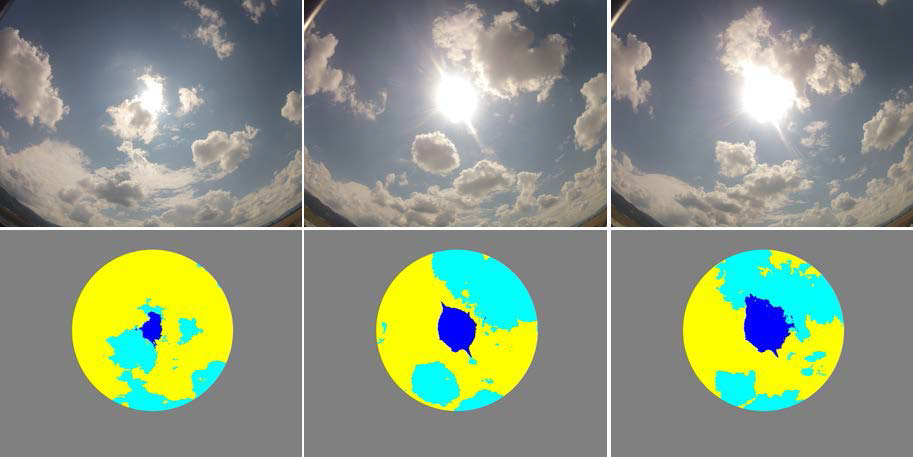
\includegraphics[scale=.5]{capatitati}
\centering
\end{figure} 

 The irradiance (direct, diffuse, global) is recorded using the equipment Kipp \& Zonen, Solys2 at the same time of image capturing. Finally, a regressor used to estimate direct irradiation (DNI) based on a feature vector consisting the number of pixels of different zone types in the images. The correlation in the result is shown in figure\ref{fig:w1_predict}.

\begin{figure}[h]
\caption{Correlation between estimated DNI and recorded DNI.}
\label{fig:w1_predict}
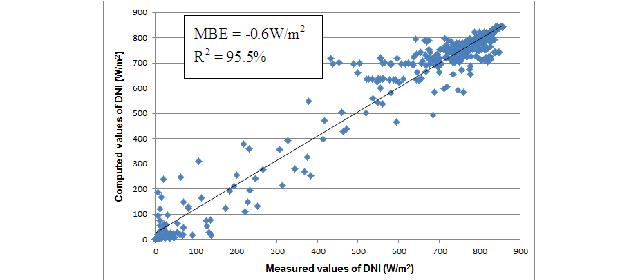
\includegraphics[scale=.7]{w1_predict}
\centering
\end{figure} 

\section{Using clear sky irradiance model and binary cloud mask}
The work done by T. Schmidt et al.\cite{tSchmidt_full} at University of Oldenburg in Germany is a very recent and relevant work on irradiance forecast using sky imager pictures. The experimental setup consists of a wide-view camera, one ceilometer (cloud base height sensor) located next to the camera, and a grid of 99 pyranometer distributed uniformly over 10km by 12km in the area close to camera. The aim is to forecast irradiance of every pyranometer up to 30 minutes. The training data is recorded from the pyranometers and the camera for two months every 10 seconds during daytime.
In order to determine clouds projection on the ground, they apply a series of image processing algorithms. 
\subsection{Cloud detection}
Firstly, they use Red-to-Blue Ratio (RBR) threshold for cloud detection which was first developed by Scripps Institution of Oceanography \cite{RBR89, RBR98} and is been used in many sky-imager-based forecast applications such as \cite{cloud_detection_using_RBR}.  The RBR values close to 1 are usually cloud, and values very less than 1 are blue sky, since the blue channel which is in denominator dominates the red channel. However, since the RBR is not homogeneously distributed over the whole field of view, using a fixed global threshold for cloud detection brings a lot of misclassification for the areas close to the sun and also dark thick clouds or very transparent clouds. Therefore, they correct the RBR values based on clear-sky RBR values for each pixel. A Clear Sky Library (CSL) is created from images of one clear day. Then, the closest distance of current position and sun positions of CSL images is used to choose the reference RBR image map. This RBR map is used in correction formula \ref{eq:RBR_correction} to decrease RBR threshold in circumsolar area to counter effect of sun saturation there. The correction also decreases RBR threshold for dark areas and increases it for bright pixels of image in order to detect thick and thin clouds.
\begin{equation}
\label{eq:RBR_correction}
R_{mod,i,j} =  R_{orig,i,j} - R_{CSL,i,j} \times (a \times S - b \times (I_{i,j} - 200))
\end{equation}
Where $0<S<1$ is the average pixel intensity in circumsolar area.

\subsection{Image un-distorion}
Since the raw image is from a fisheye lens, they apply a transformation to project it into geometric coordinates for convenience in other calculations. For that, intrinsic parameters of camera are determined using Scaramuzza Matlab toolbox \cite{fisheye_undistort} which solves a fifth-degree polynomial function of point-mapping between fisheye image and plain image. The extrinsic parameters are calculated as the best rotation which matches position of sun re-projection (derived mathematically) and sun position in the image. They calculate sun zenith and azimuth by using solar geometry2 algorithm\cite{sun_pos1}.

\subsection{Shadow mapping}
In this step, shadow of cloud pixels are projected on the ground. For this, besides incidence and azimuth angle of every cloud pixel (which is derived using camera calibration function), cloud base height is needed. The cloud base height is estimated using a ceilometer for every point in time. However, to smooth th data, median of last 30 measurements is used. Even though the ceilometer supports multi-layer clouds as well, in this work they only use the lower-level cloud height. The distance of every cloud pixel to the camera is derived using $d_{i,j} = h \times tan(\theta_{i,j})$. Given the distance $d_{i,j}$, incidence angle $\theta{i,j}$, pixel's azimuth angle $\phi_{i,j})$ and current sun position angles, horizontal distance of the cloud's show on the ground from the camera is calculated using Eq. \ref{eq:shadow_map}.
\begin{equation}
\label{eq:shadow_map}
\begin{split}
dx_{i,j} = h \times tan(\theta_{i,j}) \times sin(\phi_{i,j}) + h \times  tan(\theta_{sun}) \times sin(\phi_{sun}) \\
dy_{i,j} = h \times tan(\theta_{i,j}) \times cos(\phi_{i,j}) + h \times  tan(\theta_{sun}) \times cos(\phi_{sun})
\end{split}
\end{equation}


irradiance retrieval using K* histograms of irradiation past 30 min using clear sky data reference as normalizer

cloud motion vector using standard optical flow. cloud edges and corners in past 2 min.
ray tracing to map new cloud state on ground and forecast irradiance.
grid of pyranometers for evaluating effects of using only one pyranometer next to camera
compare forecast skill to persistent model (mention persistent model)
compare forecast skill in different cloud types



\section{Retrieval of direct and diffuse irradiance from sky images}
In another recent work, T. Schmidt et al.\cite{tSchmidt15} aim to estimate components of irradiance (direct, diffuse) from the sky images.